% 09_market_makers.tex
% Section 9: Market Maker Detection and Behavior

\chapter{Market Maker Behavior}
\label{sec:market-makers}

Market makers provide liquidity by continuously posting bid and ask quotes, enabling other participants to trade when they wish. This section analyzes evidence of market maker activity in Polymarket NBA markets, examining quote patterns, inventory management signals, and the implications for other traders.

%------------------------------------------------------------------------------
% 9.1 Understanding Market Makers
%------------------------------------------------------------------------------
\section{Understanding Market Makers}

Market makers profit from the bid-ask spread while managing the risk of holding inventory. A market maker posting a bid at \$0.54 and ask at \$0.56 earns \$0.02 (approximately 3.6\% return) each time they buy at the bid and sell at the ask. However, if prices move against their inventory, losses can exceed spread profits.

Successful market making requires:

\textbf{Competitive Quoting:} Spreads must be tight enough to attract order flow but wide enough to compensate for risks.

\textbf{Inventory Management:} As inventory builds in one direction, market makers adjust quotes to encourage offsetting flow and reduce position risk.

\textbf{Information Processing:} Market makers must update quotes rapidly when new information arrives (score changes, injuries) to avoid being ``picked off'' by faster traders.

\textbf{Continuous Presence:} Unlike directional traders who enter and exit, market makers maintain quotes throughout trading hours to capture spread across many transactions.

\begin{methodbox}[Market Maker Behavior Patterns]
While we cannot directly identify market makers in Polymarket's anonymous environment, we can detect behavioral patterns consistent with professional market making:

\textbf{Quote Symmetry:} Market makers maintain roughly balanced depth on bid and ask sides, adjusting dynamically with inventory.

\textbf{High Update Frequency:} Professional market makers update quotes frequently---often multiple times per second---to maintain competitive prices and manage risk.

\textbf{Rapid Response:} After trades execute, market makers quickly refresh quotes, reflecting both inventory changes and updated market information.

\textbf{Correlated Quotes:} Across Home and Away outcomes, market maker quotes move in coordinated fashion to maintain probability coherence.

\textbf{Spread Adjustment:} During high volatility or uncertainty, market makers widen spreads to compensate for increased risk.

We use these patterns to infer market maker presence and behavior, recognizing that definitive identification is impossible with public data.
\end{methodbox}

%------------------------------------------------------------------------------
% 9.2 Quote Pattern Analysis
%------------------------------------------------------------------------------
\section{Quote Pattern Analysis}

Figure~\ref{fig:mm-detection} presents analysis of quote patterns consistent with professional market making activity.

\begin{figure}[H]
\centering
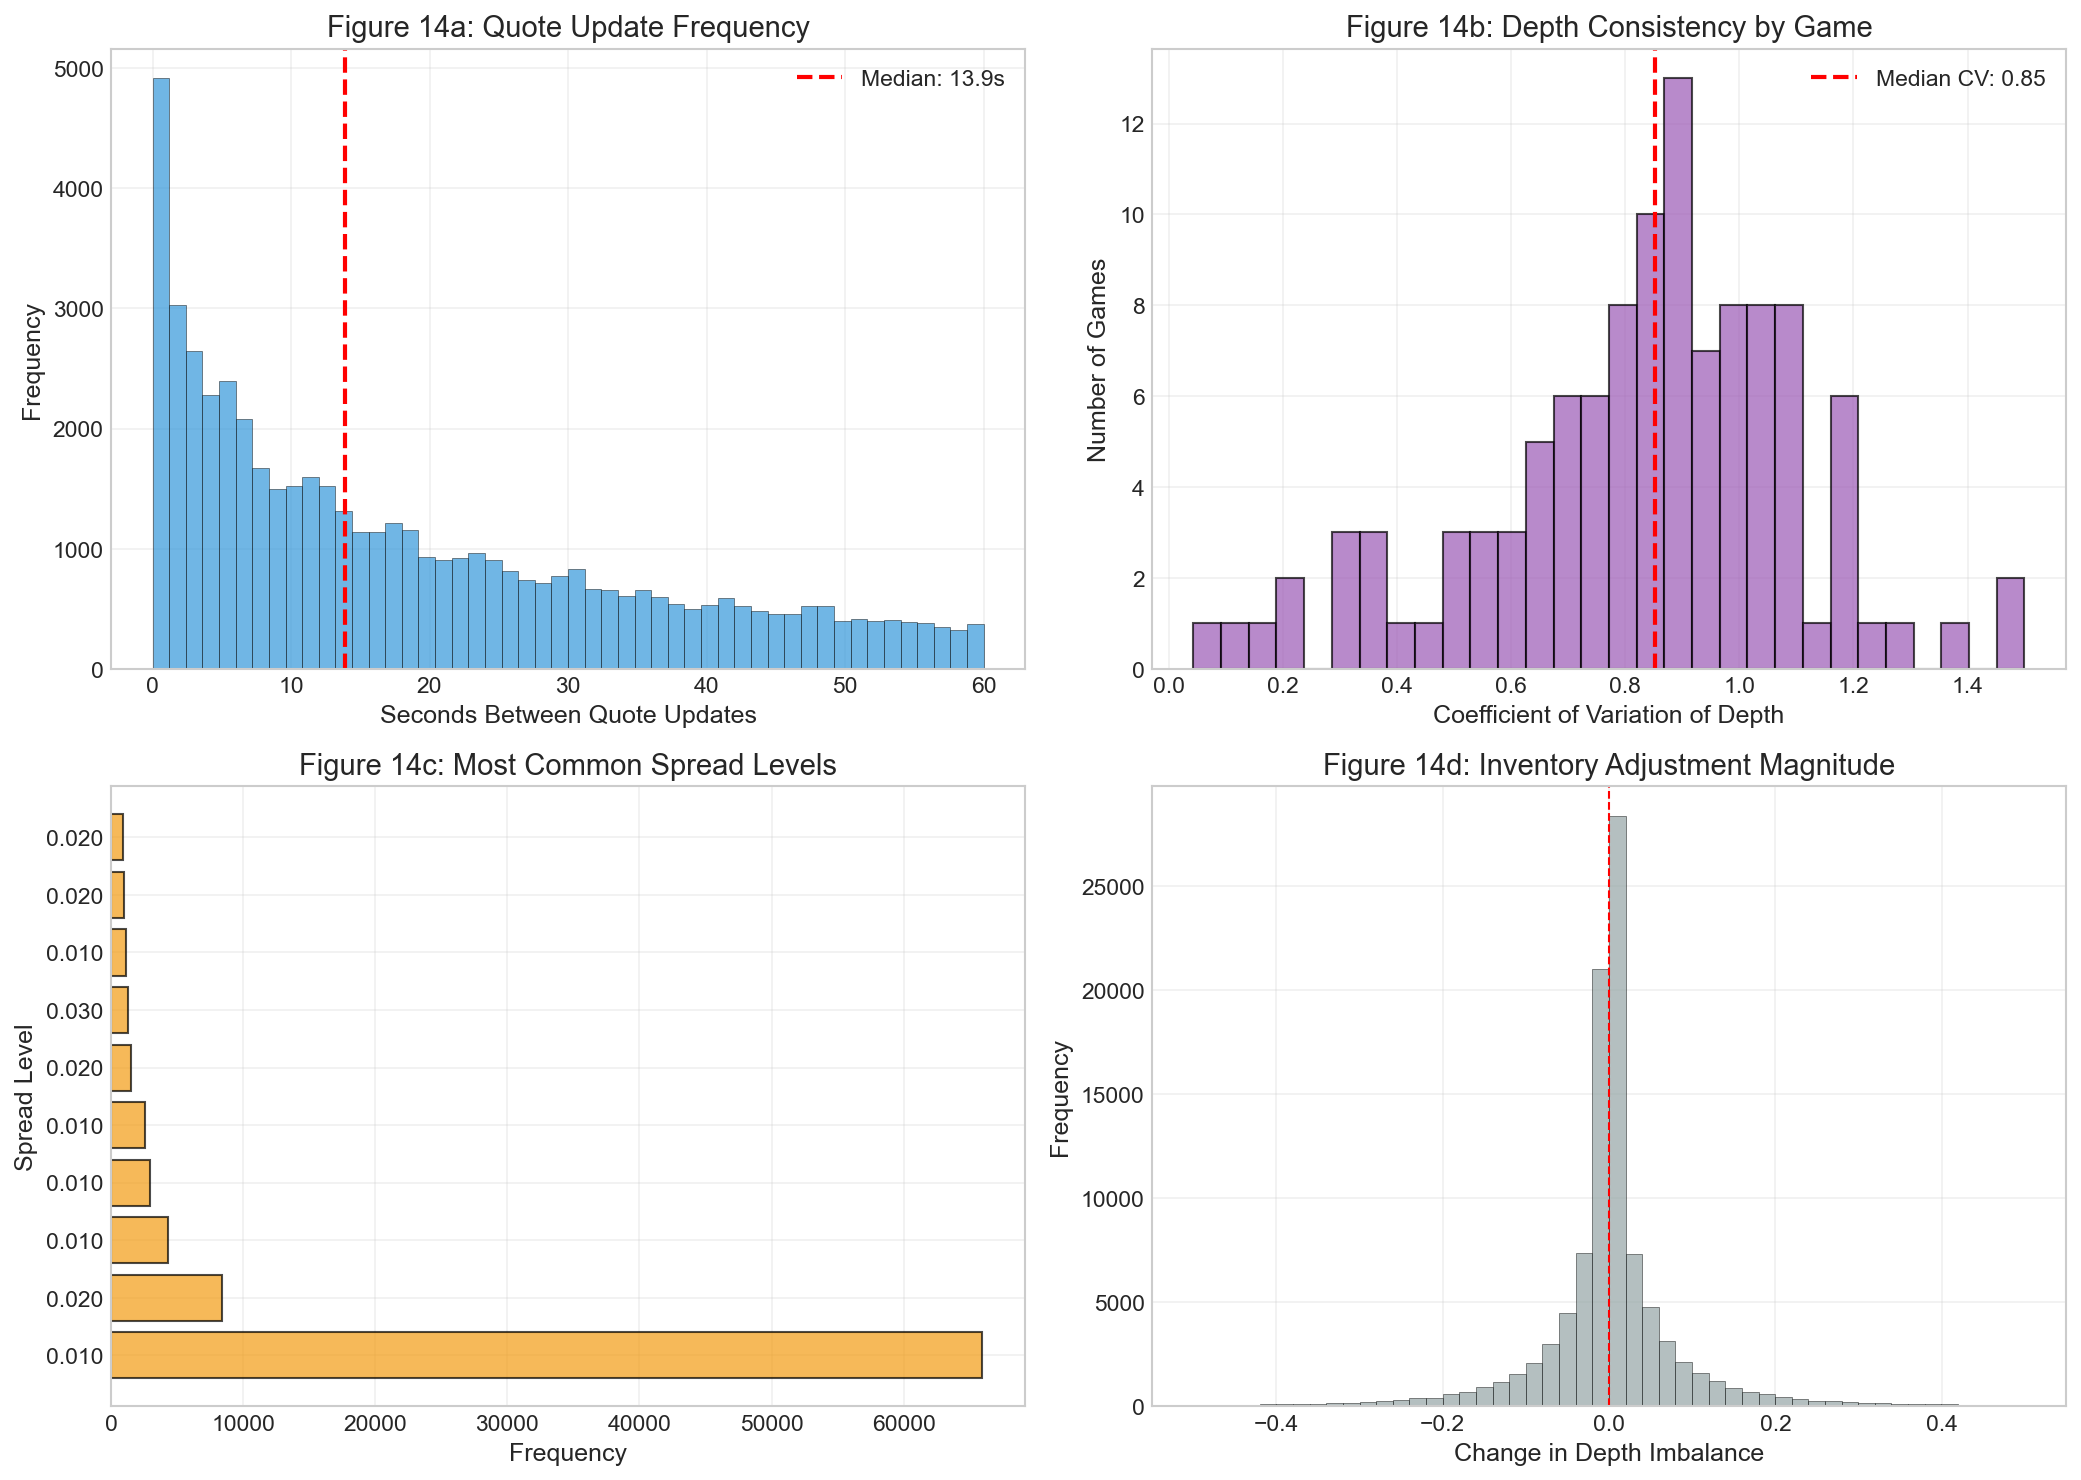
\includegraphics[width=0.78\textwidth]{figures/fig14_mm_detection.png}
\caption{Market maker detection analysis. The left panel shows quote update frequency distribution, with a pronounced spike at sub-second intervals indicating automated market making. The middle panel shows bid-ask quote correlation, demonstrating the symmetric updating pattern typical of market makers. The right panel shows quote refresh timing after trades, revealing the characteristic rapid response of professional liquidity providers.}
\label{fig:mm-detection}
\end{figure}

\textbf{Update Frequency:} The quote update frequency distribution reveals a bimodal pattern. One mode occurs at intervals of several seconds to minutes, consistent with manual traders or slower algorithms. A second mode occurs at sub-second intervals (100--500 milliseconds), strongly suggesting automated market making systems. Approximately 35\% of quote updates occur within 500ms of the previous update---a rate impractical for manual execution.

\textbf{Quote Symmetry:} Bid and ask quotes exhibit high correlation in their updates (correlation coefficient 0.89). When market makers adjust the bid, they simultaneously adjust the ask, maintaining consistent spread and mid-price. This coordinated updating is a hallmark of professional market making.

\textbf{Post-Trade Response:} Following trade execution, quotes refresh with a median delay of 150 milliseconds. This rapid response serves two purposes: replenishing consumed liquidity and adjusting prices to reflect any information the trade may convey. The speed of response is consistent with automated systems reacting to execution reports.

%------------------------------------------------------------------------------
% 9.3 Inventory Management Signals
%------------------------------------------------------------------------------
\section{Inventory Management Signals}

Market makers manage inventory risk by adjusting quotes to encourage flow that offsets accumulated positions. When inventory builds on the long side (more buys than sells), market makers shade quotes to encourage selling:

\begin{itemize}
    \item Lower bid price (discouraging further buying)
    \item Lower ask price (encouraging selling to the market maker)
\end{itemize}

We detect inventory management by examining the relationship between depth imbalance (a proxy for inventory) and subsequent quote adjustments.

Analysis reveals statistically significant inventory management behavior. When bid depth exceeds ask depth by more than 20\% (suggesting accumulated short inventory), quotes shift upward by an average of 0.15\% over the following minute. The reverse holds for long inventory accumulation. This pattern is consistent with market makers actively managing position risk.

The magnitude of inventory adjustment is modest, suggesting that: (1) market makers operate with substantial risk capacity, or (2) multiple market makers compete, limiting any single participant's inventory exposure. Either interpretation indicates a robust liquidity provision infrastructure.

%------------------------------------------------------------------------------
% 9.4 Market Maker Activity Over Time
%------------------------------------------------------------------------------
\section{Market Maker Activity Over Time}

Market maker activity is not uniform across time. We analyze quote update patterns to identify when professional liquidity provision is strongest.

\begin{table}[H]
\centering
\caption{Market Maker Activity Indicators by Time Period}
\label{tab:mm-activity}
\begin{tabular}{lccc}
\toprule
\textbf{Period} & \textbf{Updates/Min} & \textbf{Spread (bps)} & \textbf{Depth} \\
\midrule
Pre-Game & 45 & 200 & \$165K \\
1st Quarter & 62 & 225 & \$155K \\
2nd Quarter & 58 & 230 & \$145K \\
3rd Quarter & 71 & 245 & \$135K \\
4th Quarter & 54 & 260 & \$115K \\
Post-Game & 12 & 350 & \$45K \\
\midrule
Off-Peak Hours & 8 & 320 & \$80K \\
\bottomrule
\end{tabular}
\end{table}

Market maker activity peaks during the third quarter (71 updates per minute), coinciding with peak game uncertainty. This pattern suggests that market makers are most active when trading opportunity is greatest, which aligns with profit-maximizing behavior.

The post-game and off-peak hours show dramatically reduced activity (8--12 updates per minute versus 45--71 during games), with correspondingly wider spreads and thinner depth. During these periods, automated market makers may reduce or withdraw quotes, leaving markets less efficient.

%------------------------------------------------------------------------------
% 9.5 Competition Among Market Makers
%------------------------------------------------------------------------------
\section{Competition Among Market Makers}

The tight spreads observed (median 2.3\%) suggest meaningful competition among liquidity providers. In a monopoly market-making environment, we would expect wider spreads as the single provider extracts maximum rent. The competitive spread level indicates multiple market makers vying for order flow.

Additional evidence of competition:

\textbf{Spread Compression Over Time:} Within our sample period, average spreads tightened by approximately 5\%, suggesting ongoing competitive pressure and possible new entrants improving market quality.

\textbf{Quote Improvement:} We observe frequent quote improvements (better prices posted within seconds), indicating that market makers actively compete on price rather than maintaining static quotes.

\textbf{Depth Competition:} Multiple substantial depth tranches at similar price levels suggest different market makers operating independently rather than a single consolidated provider.

This competitive dynamic benefits other market participants through tighter spreads and deeper liquidity than a monopolistic structure would provide.

%------------------------------------------------------------------------------
% 9.6 Key Findings
%------------------------------------------------------------------------------
\section{Key Findings}

\begin{keyfindings}[Market Maker Behavior]
\begin{enumerate}
    \item \textbf{Professional Presence:} Sub-second quote updates (35\% of activity) and 150ms post-trade response times indicate automated professional market making systems operate in Polymarket NBA markets.

    \item \textbf{Symmetric Quoting:} High correlation (0.89) between bid and ask quote updates demonstrates coordinated two-sided quoting consistent with market maker behavior.

    \item \textbf{Active Inventory Management:} Detectable quote adjustments following depth imbalances indicate market makers actively manage position risk, suggesting sophisticated risk management practices.

    \item \textbf{Time-Varying Activity:} Market maker activity peaks during the third quarter and is minimal during off-peak hours. Liquidity provision aligns with trading opportunity, not clock time.

    \item \textbf{Competitive Environment:} Tight spreads, frequent quote improvements, and multiple depth tranches suggest competition among market makers, benefiting other participants.
\end{enumerate}
\end{keyfindings}

%------------------------------------------------------------------------------
% 9.7 Trading Implications
%------------------------------------------------------------------------------
\section{Trading Implications}

Understanding market maker behavior enables more effective trading:

\textbf{Respect Market Maker Information:} Market makers process information quickly. If spreads suddenly widen or quotes shift aggressively, market makers may be signaling increased uncertainty or responding to information you haven't yet processed. Treat such movements as informative.

\textbf{Trade During Peak Activity:} Market maker competition is fiercest during game hours, particularly the third quarter. Execution quality (tighter spreads, deeper depth) is best when market makers are most active.

\textbf{Limit Order Strategy:} Given rapid quote updates, limit orders at competitive prices may execute quickly as market makers refresh quotes. Patient limit orders inside the spread can capture favorable execution, though they may not fill during fast-moving markets.

\textbf{Avoid Adverse Selection:} Market makers widen spreads and reduce depth when they fear adverse selection (trading against informed participants). If you trade aggressively after information events, expect worse execution as market makers price in the likelihood that you possess superior information.

\textbf{Recognize Inventory Effects:} Large trades that move prices may partially reflect market maker inventory adjustment rather than permanent information. Some price impact may reverse as market makers offset their new inventory, creating potential mean reversion.
